\section{ Bayesian Filter for Tracking Moo-Deng's Behavior I (32)}

\begin{figure}[H]
    \centering
    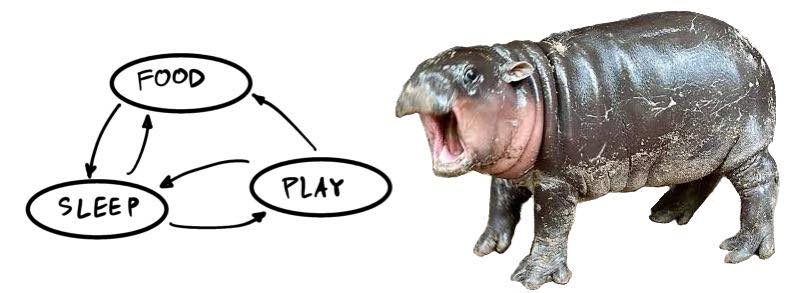
\includegraphics[width=0.65\textwidth]{img/moodeng.jpg}
    \caption{An abstract version of Moo-Deng's enclosure}
    \label{fig:p3c1}
\end{figure}

Khao Kheow Open Zoo in Thailand has gained popularity thanks to its star resident, Moo-Deng, a playful yet feisty Pygmy hippo. To better understand Moo-Deng's daily routine, the zoo has hired a wildlife researcher to track her movements between three key zones: Feeding Area ($A=1$), Resting Area ($A=2$),Playground Area ($A=3$).
Let $\mathbf{x}$ be a vector of probability of Moo-Deng being in the feeding area, the resting area, and the playground area respectively, which can be formally expressed as follows:
\begin{equation*}
    \mathbf{x}=\begin{bmatrix}
    p(A=1) \\ p(A=2) \\ 
    p(A=3)   
    \end{bmatrix}
\end{equation*}
It can be assumed that Moo-Deng only stays in one of these 3 places. Therefore:
\begin{equation*}
\sum_{i=1}^3p(A=i)=\mathbf{1}^\top\mathbf{x}=1
\end{equation*}
After careful observation, the researcher has identified Moo-Deng's behavior patterns:
\begin{itemize}
    \item When Moo-Deng is in the Feeding Area ($A=1$), she has a 60\% chance of staying there, and  a 40\% chance of moving to the Resting Area ($A=2$).
    \item If Moo-Deng is in the Resting Area ($A=2$), she has a 40\% chance of staying there, a 20\% chance of returning to the Feeding Area ($A=1$), and a 40\% chance of moving to the Playground Area ($A=3$).
    \item If Moo-Deng is in the Playground Area ($A=3$), she has a 70\% chance of staying there, a 20\% chance of moving to the Feeding Area ($A=1$), and a 10\% chance of moving to the Resting Area ($A=2$).
\end{itemize}
The behavior of Moo-Deng can be modelled as a transition matrix $\mathbf{A}\in\mathbb{R}^{3\times3}$ such that the following is true:
\begin{equation*}  \mathbf{x}_{k+1}=\mathbf{A}\mathbf{x}_{k}
\end{equation*}
where $\mathbf{x}_k$ denotes the probability vector at the $k^\text{th}$ observation.

Furthermore, the researcher uses a digital sensor system to track Moo-Deng’s location, but the sensor is not perfectly accurate:
\begin{itemize}
    \item When Moo-Deng is in the Feeding Area, the sensor reports Feeding Area with an 80\% accuracy, but it incorrectly reports Resting Area 10\% of the time and Playground Area 10\% of the time.
    \item When Moo-Deng is in the Resting Area, the sensor reports Resting Area 70\% of the time, but it incorrectly reports Feeding Area 20\% of the time and Playground Area 10\% of the time.
    \item When Moo-Deng is in the Playground Area, the sensor reports Playground Area with an 85\% accuracy, but it incorrectly reports Resting Area 10\% of the time and Feeding Area 5\% of the time.
\end{itemize}
At the $k^\text{th}$ observation, the reading from the sensor system can be encoded to a vector of digital values $\mathbf{y}_k$ so that:
\begin{equation*}
    \mathbf{y}_k=\begin{cases}
        \begin{bmatrix}
            1 & 0 & 0
        \end{bmatrix}^\top & \text{if} \quad\text{the measurement displays \texttt{Feeding Area}}\\
        \begin{bmatrix}
            0 & 1 & 0
        \end{bmatrix}^\top & \text{if} \quad\text{the measurement displays \texttt{Resting Area}}\\
        \begin{bmatrix}
            0 & 0 & 1
        \end{bmatrix}^\top & \text{if} \quad\text{the measurement displays \texttt{Playground Area}}
    \end{cases}    
\end{equation*}
Then, the probaiblity of sensor displaying each area can be modelled as follows:

\begin{equation*}
    \begin{bmatrix}
        p(\mathbf{y}_k=\begin{bmatrix}
            1 & 0 &0
        \end{bmatrix}^\top)\\
        p(\mathbf{y}_k=\begin{bmatrix}
            0 & 1 &0
        \end{bmatrix}^\top)\\
        p(\mathbf{y}_k=\begin{bmatrix}
            0 & 0 &1
        \end{bmatrix}^\top)
    \end{bmatrix}=\mathbf{C}\mathbf{x}_k
\end{equation*}
where $\mathbf{C}\in\mathbb{R}^{3\times3}$ is yet to be determined.

\begin{enumerate}[a)]
    \item Assume that Moo-Deng starts in the Feeding Area ($A_0=1$). What is the probability that her subsequent movements will follow the sequence ($2$,$3$,$3$,$1$) in this exact order? Explain your calculation. [4 pts]
    
    \textbf{Answer}: \\
    To find the probability that Moo-Deng follows the sequence $(2, 3, 3, 1)$, starting in the Feeding Area, we multiply the conditional probabilities of each step as follows:
    
    \begin{itemize}
        \item Step 1: The conditional probability of moving to \(A=2\) given the current state is \(A=1\) is \(\textbf{40}\%\).
        \item Step 2: The conditional probability of moving to \(A=3\) given the current state is \(A=2\) is \(\textbf{40}\%\).
        \item Step 3: The probability of staying in \(A=3\) is \(\textbf{70}\%\).
        \item Step 4: The conditional probability of moving to \(A=1\) given the current state is \(A=3\) is \(\textbf{20}\%\).
    \end{itemize}
    
    The probability that Moo-Deng follows the sequence $(2, 3, 3, 1)$, starting in the Feeding Area is:
    \[
    0.4 \times 0.4 \times 0.7 \times 0.2 = 0.0224 = \bm{2.24\%}
    \]
    \item Determine the numerical value of the transition matrix $\mathbf{A}$. You must explain your rationale. [5 pts]
    
    \textbf{Answer}: \\
    The transition matrix $\mathbf{A}$ describes the probability of transitioning from one area to another and can be understood from the total probability equation:

    \[
    p(A_{k+1} = i) = \sum_{j=1}^3 P(A_{k+1} = i \mid A_k = j) \cdot p(A_k = j)
    \]
    Given this equation for applying state transitions: $\mathbf{x}_{k+1}=\mathbf{A}\mathbf{x}_{k}$, it is evident that the $A$ matrix should be constructed like so:
    \[
    \mathbf{A} = \begin{bmatrix}
    P(A_{k+1}=1 \mid A_k=1) & P(A_{k+1}=1 \mid A_k=2) & P(A_{k+1}=1 \mid A_k=3) \\
    P(A_{k+1}=2 \mid A_k=1) & P(A_{k+1}=2 \mid A_k=2) & P(A_{k+1}=2 \mid A_k=3) \\
    P(A_{k+1}=3 \mid A_k=1) & P(A_{k+1}=3 \mid A_k=2) & P(A_{k+1}=3 \mid A_k=3)
    \end{bmatrix}
    \]

    When Moo-Deng is in the Feeding Area ($A_k=1$), she has a 60\% chance of staying there ($A_{k+1} = 1$), and  a 40\% chance of moving to the Resting Area ($A_{k+1}=2$).
    \begin{itemize}
            \item $P(A_{k+1}=1 \mid A_k=1) = 0.6$.
            \item $P(A_{k+1}=2 \mid A_k=1) = 0.4$.
            \item $P(A_{k+1}=3 \mid A_k=1) = 0.0$.
        \end{itemize}
If Moo-Deng is in the Resting Area ($A_k=2$), she has a 40\% chance of staying there ($A_{k+1} = 2$), a 20\% chance of returning to the Feeding Area ($A_{k+1}=1$), and a 40\% chance of moving to the Playground Area ($A_{k+1}=3$).
       \begin{itemize}
            \item $P(A_{k+1}=1 \mid A_k=2) = 0.2$.
            \item $P(A_{k+1}=2 \mid A_k=2) = 0.4$.
            \item $P(A_{k+1}=3 \mid A_k=2) = 0.4$.
        \end{itemize}
        
If Moo-Deng is in the Playground Area ($A_k=3$), she has a 70\% chance of staying there ($A_{k+1} = 3$), a 20\% chance of moving to the Feeding Area ($A_{k+1}=1$), and a 10\% chance of moving to the Resting Area ($A_{k+1}=2$).
         \begin{itemize}
            \item $P(A_{k+1}=1 \mid A_k=3) = 0.2$.
            \item $P(A_{k+1}=2 \mid A_k=3) = 0.1$.
            \item $P(A_{k+1}=3 \mid A_k=3) = 0.7$.        
        \end{itemize}


    
    Thus, we have:
    \[
    \mathbf{A} = \begin{bmatrix} 
    0.6 & 0.2 & 0.2 \\ 
    0.4 & 0.4 & 0.1 \\ 
    0.0 & 0.4 & 0.7 
    \end{bmatrix}
    \]
    \item Analytically compute the stationary probabilities of Moo-Deng’s location $\mathbf{x}^*$. These are the probabilities that, after many transitions, Moo-Deng will be found in each of the zones regardless of the initial location. You must show your work. [Hint: $??=\mathbf{A}\mathbf{x}^*$] [8 pts]
    
    \textbf{Answer}: \\
    The stationary vector $\mathbf{x}^* = \begin{bmatrix} x_1^* & x_2^* & x_3^* \end{bmatrix}^\top$ represents the long-term probabilities that Moo-Deng will be in each area, and it satisfies:
    \[
    \mathbf{x}^*_{k+1} = \mathbf{A} \mathbf{x}^*_k
    \]
    while being constrained by the following:
    \[
    x_1^* + x_2^* + x_3^* = 1.
    \]
    which makes intuitive sense since it means that at this point in the transition of the state, the next state will not be different than the previous state, suggesting that the probabilities are 'stationary'.
    
    Expanding $\mathbf{x}^* = \mathbf{A} \mathbf{x}^*$ gives a system of linear equations:
    
    \begin{align*}
        0.6 x_1^* + 0.2 x_2^* + 0.2 x_3^* &= x_1^* \\
        0.4 x_1^* + 0.4 x_2^* + 0.1 x_3^* &= x_2^* \\
        0.4 x_2^* + 0.7 x_3^* &= x_3^*
    \end{align*}
    
Using the equations above along with the provided constraint, we get the following result for $\mathbf{x}^*$:
\[
\mathbf{x}^* = \begin{bmatrix} \frac{1}{3} & \frac{2}{7} & \frac{8}{21} \end{bmatrix}^\top
\]
    \item Determine the numerical value of the  matrix $\mathbf{C}$. You must explain your rationale. [5 pts] \\
    \textbf{Answer}:

    The matrix $\mathbf{C}$ models the sensor's measurement probabilities for each of the three areas (Feeding Area, Resting Area, and Playground Area), based on the current state. To determine $\mathbf{C}$, we need to use the sensor accuracy and error rates provided. \\
\textbf{Sensor Accuracy and Error Rates:}

\begin{itemize}
    \item When Moo-Deng is in the Feeding Area, the sensor reports Feeding Area with an 80\% accuracy, but it incorrectly reports Resting Area 10\% of the time and Playground Area 10\% of the time.
    \begin{itemize}
        \item $P(\mathbf{y}_k = [1, 0, 0]^\top \mid A=1) = 80\%$
        \item $P(\mathbf{y}_k = [0, 1, 0]^\top \mid A=1) = 10\%$
        \item $P(\mathbf{y}_k = [0, 0, 1]^\top \mid A=1) = 10\%$
    \end{itemize}
    \item When Moo-Deng is in the Resting Area, the sensor reports Resting Area 70\% of the time, but it incorrectly reports Feeding Area 20\% of the time and Playground Area 10\% of the time.
    \begin{itemize}
        \item $ P(\mathbf{y}_k = [1, 0, 0]^\top \mid A=2) = 20\%$
        \item $P(\mathbf{y}_k = [0, 1, 0]^\top \mid A=2) = 70\%$
        \item $P(\mathbf{y}_k = [0, 0, 1]^\top \mid A=2) = 10\%$
    \end{itemize}
    \item When Moo-Deng is in the Playground Area, the sensor reports Playground Area with an 85\% accuracy, but it incorrectly reports Resting Area 10\% of the time and Feeding Area 5\% of the time.
    \begin{itemize}
        \item $ P(\mathbf{y}_k = [1, 0, 0]^\top \mid A=3) = 5\%$
        \item $P(\mathbf{y}_k = [0, 1, 0]^\top \mid A=3) = 10\%$
        \item $P(\mathbf{y}_k = [0, 0, 1]^\top \mid A=3) = 85\%$
    \end{itemize}
\end{itemize}

\textbf{Matrix \(\mathbf{C}\):}

Matrix \(\mathbf{C}\) can be constructed by leveraging the total probability principle, similar to the construction of the $A$ matrix:


\[
\mathbf{C} = \begin{bmatrix}
P(\mathbf{y}_k = [1, 0, 0]^\top \mid A=1) 
& P(\mathbf{y}_k = [1, 0, 0]^\top \mid A=2) 
& P(\mathbf{y}_k = [1, 0, 0]^\top \mid A=3) \\
P(\mathbf{y}_k = [0, 1, 0]^\top \mid A=1) 
& P(\mathbf{y}_k = [0, 1, 0]^\top \mid A=2)
& P(\mathbf{y}_k = [0, 1, 0]^\top \mid A=3) \\
P(\mathbf{y}_k = [0, 0, 1]^\top \mid A=1)
& P(\mathbf{y}_k = [0, 0, 1]^\top \mid A=2)
& P(\mathbf{y}_k = [0, 0, 1]^\top \mid A=3)
\end{bmatrix}
\]

Substituting the values from above:
\[
\mathbf{C} = \begin{bmatrix}
0.8 & 0.2 & 0.05 \\
0.1 & 0.7 & 0.1 \\
0.1 & 0.1 & 0.85
\end{bmatrix}
\]
    \item Derive a state estimator based on a Bayesian Filter that estimates the states and probability of Moo-Deng's  based on prior belief $\mathbf{x}_{k-1}$ and the current sensor measurement $\mathbf{y}_k$. You may leave your answer in terms of $\mathbf{A}$ and $\mathbf{C}$. You may also substitute their numeric values. [10 pts] \\
    \textbf{Answer}: \\
    Bayesian Filter for State Estimation (Prediction Step):
\begin{equation}
    \overline{bel}(x_k) = \sum p(x_k | x_{k-1}) \, bel(x_{k-1})
\end{equation}
Bayesian Filter for State Estimation (Correction Step): \\
\begin{equation} bel(x_k) = \eta p(y_k | x_k) \, \overline{bel}(x_k) \end{equation}
In the context of this problem, $bel(\bm{x}_k)$ will be a $3 \times 1$ vector with 3 potential values (the same potential values as $y_k$: 
        $\begin{bmatrix}
            1 & 0 & 0
        \end{bmatrix}^T$,
        $\begin{bmatrix}
            0 & 1 & 0
        \end{bmatrix}^T$, $\begin{bmatrix}
            0 & 0 & 1
        \end{bmatrix}^T$), 
which represents the best guess of Moo-Deng's current state/location. \\

Conditional probability of the current state given the previous state, $p(x_k | x_{k-1})$, is captured by the $\bm{A}$ matrix. Thus, the $\bm{A}$ matrix can be substituted into equation (1) in place of the $\sum p(x_k | x_{k-1})$

\begin{equation}
    \overline{bel}(\bm{x}_k) = \bm{A} \cdot bel(\bm{x}_{k-1})
\end{equation}

Conditional probability of the current measurements given the current state, $p(y_k | x_k)$, is captured by the $\bm{C}$ matrix. Thus, the $\bm{C}$ matrix can be substituted into equation (2) in place of the $p(y_k | x_k)$
\begin{equation}
    bel(\bm{x}_k) = \eta \bm{C} \cdot \overline{bel}(\bm{x}_k)
\end{equation}
Combining equations (3) and (4) and dropping the normalization factor $\eta$ for clarity:
\begin{equation}
    bel(\bm{x}_k) = \bm{C} \bm{A} \cdot bel(\bm{x}_{k-1})
\end{equation}
\end{enumerate}
